%%%% 
% This is a template for project reports in the subject DAT620 at the
% Department of Electrical Engineering and Computer Science,
% University of Stavanger.
% 
% The template is based on the ACM conference template 
% it was edited by Leander Jehl and Hein Meling
\documentclass[sigconf]{acmart}

\usepackage{listings}

\usepackage{xcolor}
\definecolor{codegreen}{rgb}{0,0.6,0}
\definecolor{codegray}{rgb}{0.5,0.5,0.5}
\definecolor{codepurple}{rgb}{0.58,0,0.82}
\definecolor{backcolour}{rgb}{1,1,1}

%Code listing style named "mystyle"
\lstdefinestyle{mystyle}{
  backgroundcolor=\color{backcolour}, commentstyle=\color{codegreen},
  keywordstyle=\color{magenta},
  numberstyle=\tiny\color{codegray},
  stringstyle=\color{codepurple},
  basicstyle=\ttfamily\footnotesize,
  breakatwhitespace=false,         
  breaklines=true,                 
  captionpos=b,                    
  keepspaces=true,                 
  numbers=left,                    
  numbersep=5pt,                  
  showspaces=false,                
  showstringspaces=false,
  showtabs=false,                  
  tabsize=2
}


%DON'T CHANGE THIS FILE
%This file sets several properties for the ACM template.
%It is not necessary to change this file.


% Copyright
\setcopyright{none}

% DOI
\acmDOI{}

% ISBN
\acmISBN{}

%Conference
\acmConference[Project in Computer Science (DAT500)]{}{}{UiS}
\acmBooktitle{}
\copyrightyear{2022}

\newcommand{\supervisors}[1]{\thanks{Supervised by #1}}


%In the preamble file you can include packages and define macros.
\usepackage{xspace}

%Here we define a marco: The \xspace ensures correct spacing, i.e. insert space before next word, but not before period or comma.
\newcommand{\paxos}{\textsc{Paxos}\xspace}

%These packages are needed for the plot in Figure 1. 
\usepackage{tikz}
\usepackage{pgfplots}
\pgfplotsset{compat=newest}



\begin{document}


%TODO: Replace the title with your project title.
\title{Amazon Customer Reviews Analysis}
%you may use a subtitle
\subtitle{A Data-Intensive System Practice}

%TODO replace author names with your name and email below:
\author{Abolfazl Taleb Zadeh}
\affiliation{University of Stavanger, Norway}
\email{a.talebzadeh@stud.uis.no}


\author{Vahid Nosratian}
\affiliation{University of Stavanger, Norway}
\email{v.nosratian@stud.uis.no}
%TODO: add the name of one or more supervisors
\supervisors{Tomasz Wiktorski}



\begin{abstract}
%The abstract lies in a different file: 
\textbf
Nowadays, data has become one of the most important role players of the industry. Considering the amount of data being generated in every second, the capability of handling this huge amount of data and converting it to a more practical format which demands a high level of expertise has been a quite challenging issue. As storing and handling this data is considerably expensive and urges a great deal of expenses to the industries, it is so important to get as much benefit as possible from the data. In this paper we try to facilitate the ingestion and analysis of a big dataset in matter of time and computation by implementing different algorithms like sentiment analysis and several queries and counting examples in Apache Hadoop and Apache Spark which are two data frameworks for handling big data.

\end{abstract}

%TODO: Replace with some keywords, relevant for your project
\keywords{Sentiment Analysis, Hadoop, Spark, map, reduce}

\maketitle

%Each section can be placed in a separate file and included by the input command.

\section{Introduction}
\label{sec:introduction}
\noindent
The traditional business industry used to be pretty much limited on the scope of both quality and quantity of the presented services because of the narrow amount of the demand and resources. However, after 4 stages of the industrial revolutions more specifically the latter, the capacity of the services disruptively expanded and electronic devices and particularly internet and following that data came to the play. As Online businesses and their services got more publicized the size of data generated by electronic devices and internet users grew bigger and bigger as the volume of data gets nearly doubled every four years [1] (fig-1) and this is going to get accelerated even more in the future. This data is assumed one of the most valuable assets of the business as it tells the story of the wins and losses and benefits and drawbacks. By going deep into the data combining them and inferring the coherence and utilizing them as the feed of new policies in the flow of the industries, the investment of handling and storing the data will eventually pay off and can take the business as far as it can get in the industry rivalry. If the volume of data is small and manageable considering the current existing hardware, implementing the calculations on the data-set is not a big deal but as soon as the amount of data increases, getting the favorable results from the data gets almost infeasible in the precise time window which is crucial as in most of the cases data has a crucial expiration date.

To convert the data into more useful form multiple layers of algorithms and processes is needed to be implemented on the raw data. For example, if the data is organized and stored in a relational database, the fields from different tables might need to be selected, combined, counted, aggregated, grouped, etc. this type of operations normally is done using SQL (structured query language). 

For example, if we assume that we have a table of the sales of a company which consists of the invoice number, date, sales person ID, product number and number of sold items and also a table for the products containing product ID and the price and in another table we have the information of the sales persons of the company by joining these three tables and grouping by the sales person ID and summing the items prices multiplied by the amount sold and finally sorting the result in descending order, we will have a list of sales persons and the total value of their sales and through that we can analyze the performance of the sale persons in a business. Or in our case, by implementing the sentiment analysis which analyzes, identifies, extracts, and quantifies current states and individual opinions [2] of the customers towards a specific product, valuable information can be derived from the data by combining the SQL queries, particular algorithms alongside with customer reviews sentiment analysis. As far as the volume of data is massive, implementing the necessary processes on the data would demand substantial amount of hardware and time. In fact, after the volume of data exceeds a limit implementing the process on a single computer within a promising period is not feasible. This is exactly where frames like Hadoop and Spark come to the picture.

\section{Background}
\label{sec:background}
In this section we try to expand the use case and define the existing data-set and go deeper in each field and then some tasks from which we will get a business intelligence insight will be explained and finally, the performance assessment which is separately done on multiple algorithms and also on different frameworks (e.g., Hadoop, Spark) will be discussed. 

\subsection{DATA-SET}
The selected data-set is more than 130 million Amazon customers reviews on roughly 35 Amazon product categories which is gathered from 1996 – 2015. It consists 15 fields:
\begin{itemize}
    \item marketplace: This fields expresses the country in which the item is sold and in this data-set it is \emph{US} for all fields
    \item review\textunderscore id: This field is the ID each review is referred to 
    \item product\textunderscore title: This field contains the title given to each product
    \item product\textunderscore category: Each product is placed under one of 35 existing product categories this field specifies this category.
    \item star\textunderscore rating: Each customer can rate product along with the comment that makes
    \item total\textunderscore vote: 
    \item vine: Review was written as part of the Vine program
    \item helpful\textunderscore votes: Each customer can vote for other reviews if they are helpful. This field is accumulation of the helpful votes each review has received.
    \item verified\textunderscore purchase: This fields tells if the review has been made by a verified purchase. Unquestionably, a review from a verified purchase is considered more valid. 
    \item review\textunderscore headline: Each review has a title chosen by the customer. This field expresses the tile for each review.
    \item review\textunderscore body: This field contains the body of the review
    \item review\textunderscore date: This is the date on which the review has been made
\end{itemize}

\subsection{BI RELATED WORKS}
To extract the proper BI strategies and analysis of the existing data, several queries has been implemented using MrJob in Hadoop and Spark. Below you can see a brief explanation for each procedure. We will go through the detail in other sections.

\subsubsection{Number of Reviews Each Year}

In this section the number of reviews made each year is counted by implementing a simple map-reduce algorithm in Hadoop. the result is saved in an output file in tab separated text-file. this result can be used to compare the amount of customers' attention to the products each for each year and get the correct perspective of the direction  the business is heading to.

\subsubsection{Number of Reviews Each Customer Has Made}

The result of this implementation can give the business a general idea of the activity of each customer. By using the result of this part the activity of each customer can be observed so that the customers can be classified into groups by the amount of activity. this can be used for targeted reviewer incentive plans and promotions.

\subsubsection{Number of Reviews for Each Month}

This is the same as number of reviews made each year with the difference that it has been made for each month and the result is much detailed. it can also be used to get some ideas about the different months of the year. for example, how the season and occasions like Christmas and summertime can effect on the number of reviews made by users.
\subsubsection{Number of Reviews for Each Product}
This section will provide the number of reviews each product has received. This can be used to learn which products has gathered more attention which can be used to find the most praised and criticised product by combining with the results from sentiment analysis. 
\subsubsection{Average Number of Reviews per Month During Each Year Also Max and Min Number of Reviews Received per Month During Each Year}
This section calculates the average of the number of reviews made per month during each year. It also calculates the the month with the maximum and the minimum value related to each year. Result of this section prepares the idea on how much reviews has been made averagely during each year. Besides, by knowing the months with the maximum and minimum number of reviews, thee most and the least busiest month of the year is known and can be used to imply some policies to fix any issues or bottlenecks causing recession in a period of time.

\subsubsection{The Months of Each Year with the Most and the Least Reviews}
This gives us the month of the year with maximum and minimum number of the reviews for each month. by knowing the months with the maximum and minimum number of reviews, the most and the least busy month of the year is known and can be used to imply some policies to fix any issues or bottlenecks causing recession in a period of time.
\subsubsection{The average starts given to each product by the reviewers}
The idea of the customer about the product is so valuable as it gives the feedback to the business about the performance of the business in different categories by assessing the degree of satisfactory of the customers. The average stars given to a product is a brilliant tool to comprehend how successful a product has been in the market to gather the attention and satisfactory of the buyers so that the company can pursue the right decision on the policies towards a particular product or even a product category. 

\subsection{Sentiment Analysis}
Computational intelligence technologies are proven to be essential competitive tools in many sectors as analytic and data science become more prevalent.
For example, data is mined for trends in business analytic to better understand consumers and improve sales and marketing. Probabilistic approaches may be used to detect patterns in data using computational intelligence technologies. These approaches usually operate with low-level data and aren't governed by absolute knowledge like standard AI methods. Furthermore, a significant quantity of data that requires analysis is now generated in textual form. Users might, for example, submit written reviews of a product or service on websites like Amazon and Airbnb. It's difficult to express data in an absolute grammar since written word is open to interpretation. Computational intelligence approaches, on the other hand, allow for such fuzziness and may be the best tool for detecting patterns in such data.

Sentiment analysis integrates multiple research fields such as natural language processing, data mining, and text mining, and is quickly gaining traction between many businesses as they pursue to integrate computational intelligence methods into their operations and shed more light on, and improve, their products and services. The purpose of sentiment analysis, often known as opinion mining, is to uncover people's written views. "What one feels about something," "personal experience, one's own emotion," "an attitude toward something," or "an opinion" all seem to be terms used to describe sentiment.

Beliefs are at the heart of essentially all human behavior and have a significant role in shaping our actions. Our views and interpretations, as well as the decisions we make, are heavily influenced by how society sees and interpret the world. As a result, when we need to make a decision, we frequently follow the opinion of others.
This is true not just for people but also for businesses. Closed-form client satisfaction surveys have traditionally been enough to determine the most important components, or features, of total customer satisfaction. Questionnaire development and implementation, on the other hand, might be costly or unavailable. In certain circumstances, governmental entities are even forbidden by law from collecting customer satisfaction surveys.

\section{Experimental Evaluation}
\label{sec:evaluation}
For implementing the algorithms on big data using Hadoop and Spark, a platform was prepared which could have a deliberate setup of multiple cluster~(namenodes and worker nodes) setups containing different hardware and software resources. This could prepare a very acceptable possibility of performing performance assessment practice on different algorithms using different cluster setup. Spark and Hadoop's performance is determined by a number of parameters, including hard disk (I/O storage), CPU, memory, network bandwidth, and other software layers that are well-configured. Building a Hadoop cluster is a difficult operation that involves careful consideration of various issues, including hardware selection, cluster sizing, and configuration[hadoop cluster].

\begin{figure}[t]
   \centering
   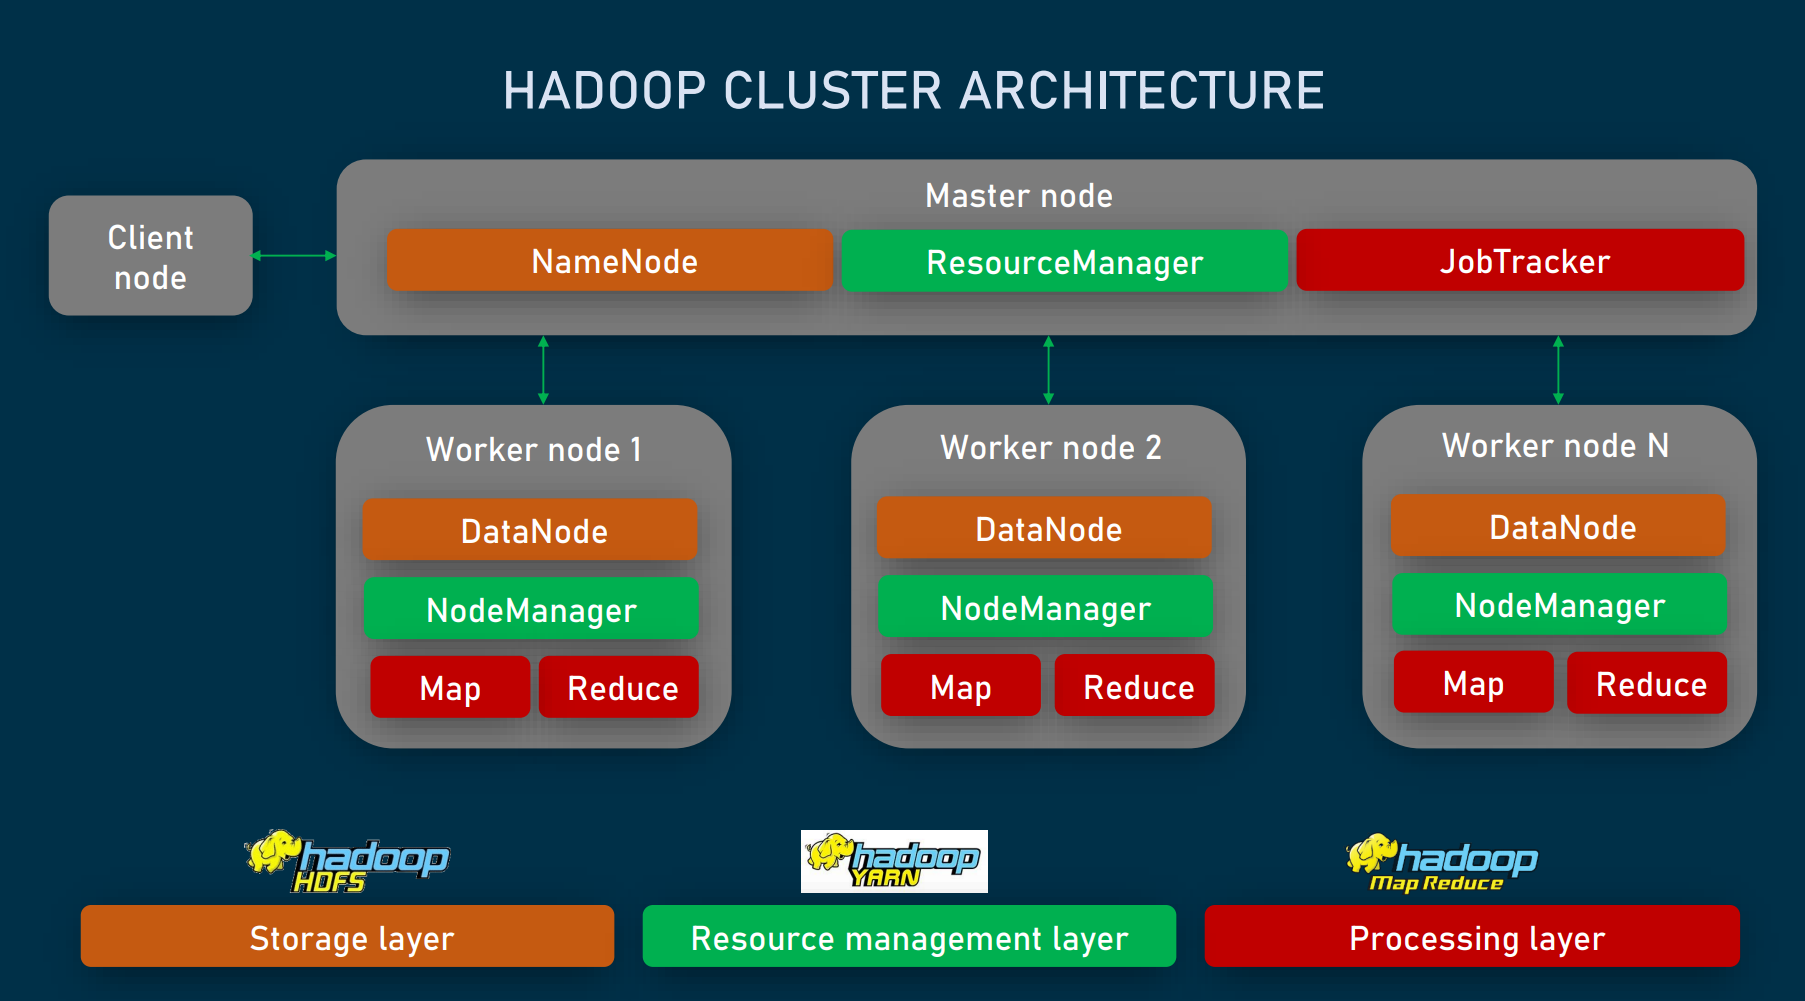
\includegraphics[width=\linewidth]{fig/hadoop_cluster.png}
    \caption{Apache Hadoop Architecture}
    \label{fig:architecture}
\end{figure}


\subsection{Experimental setup}
For this project we decided to use two different experimental setups. The primary setup contain total number of 4 nodes including one main Node and 3 data Node. The main node is named "group2" and words has been name "datanode" plus the consequent worker node order number (e.g., datanode1). All nodes had similar resources setup configuration as you can see in figure 2, there is 200~GB of HDD, 4~GB of RAM and two virtual CPU. Linux Ubuntu Forcal version 20.4 has been installed on all nodes as the operating system and Hadoop and Spark are each individually installed and configured on all nodes.
A secondary cluster configuration has also been considered which contains the same node configuration, but the total number of nodes has increased to 7 nodes including one main node and 5 worker nodes using the same naming policy.


The virtual network of the experimental setup is consisted of two networks. First one, public network and the second one group2 network which are connected together through a router.You can see the topology graph of the secondary cluster setup network on Figure~\ref{fig:topology}

\begin{figure}[t]
   \centering
   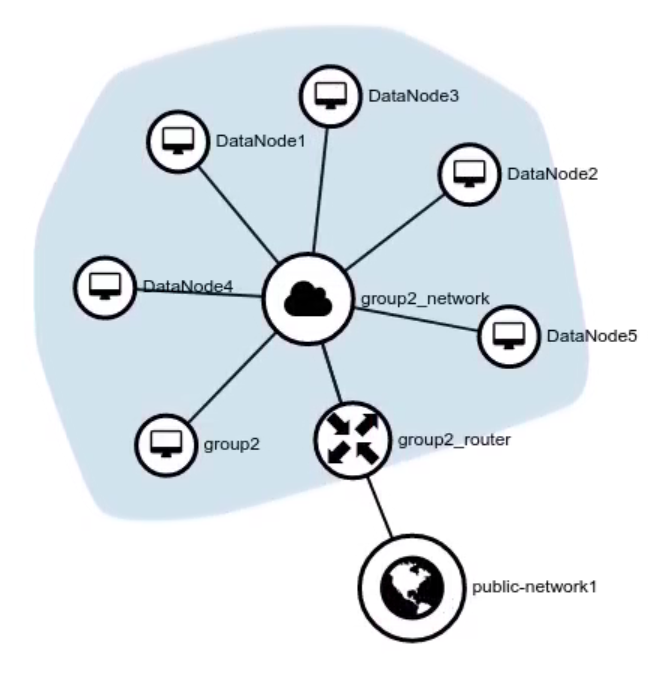
\includegraphics[width=\linewidth]{fig/NetworkTopology.png}
    \caption{Experimental Secondary Network Topology}
    \label{fig:topology}
\end{figure}

\section{Related Works}
\label{sec:relatedWorks}
The related studies which is done are mostly on sentiment analysis and its usage on developing policies for business entrepreneurs. a look through the papers leads us mostly to a list of some works done on different techniques for implementing sentiment analysis. the items below gives us an idea of what the related studies are about:
\begin{itemize}
    \item Electronic market analytic based on customer reviews: Classic challenges in e-marketing such as pricing, brand positioning and new product development are rooted in product analysis based on users’ feedback.
    \item Sentiment analysis using the product review data: Sentiment analysis also known as the emotion AI, uses natural language processing to analyze the emotions from the extracted opinions.
    \item Opinion mining and sentiment analysis on online customer review: The process of finding user opinion about the topic or product is called as opinion mining. The goal of Opinion Mining and Sentiment Analysis is to make computer able to recognize and express emotion.
    \item Classification of customer review based on the sentiment analysis: It is demonstrated that if customers' reviews are classified as negative or positive, classifications is correct with a probability of more than 90\%.
    \item The analysis and prediction of customer review rating using opinion mining in which customers commented as open opinion using probability's classifier model.
    \item Measuring e-commerce service quality from online customer review using sentiment analysis, in which more specifically the Naive Bayes classification is the most common methodology for being highly accurate and supporting big data processing.
\end{itemize}


\section{Identify Preprocessing Steps}
\label{sec:preprocessing}
Data preprocessing, which is part of data preparation, refers to any sort of processing done on raw data in order to prepare it for further processing. It has long been regarded as a crucial first stage in the data mining process. Data preparation approaches have lately been used for training machine learning and AI models, as well as for inferring against them.

Preprocessing data converts it into a format that can be handled more quickly and efficiently in data mining, machine learning, and other data science activities. To achieve reliable findings, the approaches are often utilized at the early phases of the machine learning and AI development pipeline [\ref{item:2}].

As the data that is gathered to process always is not as we anticipate, there are several preprocessing levels that needs to be done on the existing data to convert it to a more convenient form and type. below you can find multiple kinds of data preprocessing:
\begin{itemize}
    \item sampling, the process of selecting a representative selection of data from a vast population;
    \item transformation, which transforms raw data into a single output;
    \item denoising is the process of removing noise from data.
    \item imputation, which replaces missing values with statistically relevant data;
    \item normalization is the process of organizing data so that it may be accessed more quickly;
    \item feature extraction is the process of extracting a subset of relevant features that are important in a given situation.
\end{itemize}

As the data type and format is as desired in our case, there is not much necessity for preprocessing. And also as long as we are not going to do any machine learning prediction algorithms the numerical values in the data-set do not require to be watched to avoid unwanted invalid results such as division by zero and etc. On the other side, because we are doing sentiment analysis and the process requires meaningful words which can be assumed as either positive or negative. there are some text cleaning algorithms that can be useful in our case. For example, removing stop words from text can be so helpful in reducing the process time on implementing sentiment analysis. nevertheless, in the case that one of many Natural Language Processing (NLP) and more specifically Sentiment Analysis library is used, applying text cleaning (removing punctuation marks and numbers and emojis, converting to lower case and etc.) is implemented within the library and there is no need for doing any extra layer of cleaning. However, in the case of using non-trivial algorithms, applying multiple layers of text cleansing, to attain a reasonable performance threshold would be inevitable. Hence, in our case, on sentiment analysis implementation using non-trivial algorithm, all the text converted to lower case format and all non alphabetic characters are removed from the review text. This is achieved by using two methods:
\subsubsection{regEx} A regular expression (abbreviated regex or regexp; sometimes known as a rational expression) is a string of letters that defines a text search pattern. String-searching algorithms often employ such patterns for string "find" or "find and replace" operations, as well as input validation. Theoretical computer science and formal language theory have produced regular expression approaches\cite{statista}.
\subsubsection{python standard iteration and string commands}
The changes which is necessary to make the text ready for undergoing an analysis can be implemented using non-trivial algorithms. For example, in python the string can be converted to a list containing all the included letter separately, and using an iterative loop each letter can be checked, in the case that it's not in the intended format in can be excluded from the string by adding it to a new list or removing it from the original list. In code~\ref{lst:code} and code~\ref{lst:regex} you can see how python functions and regEx be utilized to cleanse a string in the proper way respectively.


\rule{200 pt}{0.5 pt} 
\renewcommand{\lstlistingname}{Code}
\lstset{style=mystyle}
\begin{lstlisting}[language=Python, caption={String cleansing using python standard functions}, label={lst:code}, mathescape = true, breaklines=true]
  #cleansing the string using python standard functions
  cleanText = ''.join(w.lower() for w in lineList[13] if w.isalpha() or w == " ")
    textList = cleanText.split(" ")
    
\end{lstlisting}

\rule{200 pt}{0.5 pt} 

\lstset{style=mystyle}
\begin{lstlisting}[language=Python, caption={String cleansing using regEx}, label={lst:regex}, mathescape = true, breaklines=true]
  #cleansing the string using regEx
  cleanText = re.sub(r"[0-9(-_:;,.!?@#%^&*)']",'',lineList[13].lower())
    textList = cleanText.split(" ")
\end{lstlisting}

\rule{200 pt}{0.5 pt} 


as the majority of the algorithms, particularly in Hadoop MRJob has been implemented in separate files and each of them uses different removing extra fields couldn't be considered as an option as for each of the algorithms one cleaning algorithm should have been implemented which imposes a very heavy over load to the system. Therefore, we decided to move on with untouched data base for running counting process in Hadoop.

\section{Related Algorithms}
\label{sec:relatedAlgorithms}
Basically, in this project multiple algorithms has been used which can be divided into two groups, the first one is the algorithms which has been used to infer some result coherence and logic to make decisions on business related acts and the second one is the algorithms which has been implemented to apply sentiment analysis on customer reviews. the first group are those which has been implemented on Hadoop and consists of 7 algorithms:
\subsection{Number of Reviews Each Year} this algorithm has been implemented using one mapper and one reducer functions. in the mapper function first, the whole line is read and sent as line into the mapper, the white spaces which is located in the beginning and at the end of the line will be dropped by using strip  python function, the stripped string then is separated and saved as a list; the 14th element of the list which is the date the review is made is selected and again separated into day, month and the year. To figure out that the date is not null or doesn't have an invalid value, within a condition, specifies if the length of separated value is equal to 3 (representing day, month and year), then the values from the first position to position number seven of the original non-separated value (to have year and month together e.g., 2002-12 for December of 2002) for date will be returned as the key and "1" as the value.

In reduce function, the list of values will be added through python function sum and is return as the value along side the key which has remained untouched from the mapper function. In code~\ref{lst:revYearCount} you see the implementation of this algorithm.




\renewcommand{\lstlistingname}{Code}
\lstset{style=mystyle}
\begin{lstlisting}[language=Python, caption={Number of Reviews Each Year}, label={lst:revYearCount}, mathescape = true, breaklines=true]
from mrjob.job import MRJob

class MRCountSum(MRJob):

    def mapper(self, _, line):
        line = line.strip()  
        lineList = line.split("\t")
        date = lineList[14]
        if len(date.split("-"))==3:
            yield date[:7],1
        yield "", 0
    def combiner(self, key, values):
        yield key, sum(values)
        
    def reducer(self, key, values):
        yield key, sum(values)

if __name__ == '__main__':
    MRCountSum.run()
\end{lstlisting}

\rule{200 pt}{0.5 pt} 


\subsection{Number of Reviews Each Customer Has Made}
The purpose of writing this algorithm has been discussed so in this part we go through the implementation and algorithm. This algorithm has been implemented using one mapper function and one reducer function. the mapper function receives the each line through line argument in the function. The line will then divided into 15 fields and stored in a list. Customer identification number is fetched from the list and stored in a variable and is returned as the key and number "1" is returned as the value to the reducer. in the reducer the unique values for each customer ID is received and the summation of number of "1" values is calculated and return to the output with the key. the code for this algorithm can be found on code~\ref{lst:CostumerCount} 

\rule{200 pt}{0.5 pt} 

\renewcommand{\lstlistingname}{Code}
\lstset{style=mystyle}
\begin{lstlisting}[language=Python, caption={Number of Reviews Each Customer Has Made}, label={lst:CostumerCount}, mathescape = true, breaklines=true]
from mrjob.job import MRJob

class MRCountSum(MRJob):

    def mapper(self, _, line):
        line = line.strip() # remove leading and trailing whitespace
        lineList = line.split("\t")
        customer = lineList[1]
        yield customer, 1
    def combiner(self, key, values):
        yield key, sum(values)
        
    def reducer(self, key, values):
        yield key, sum(values)

if __name__ == '__main__':
    MRCountSum.run()
\end{lstlisting}

\rule{200 pt}{0.5 pt} 

\subsection{Number of Reviews for Each Month}
This algorithm includes two mapper functions and two reducer functions. At the top of everything in the class    a function named steps has defined. This takes care of the order of running multiple mappers and reducers.

The first mapper function which is called "mapper\_count", receives the line as a single consistent piece of strings containing 15 values which has been put together using tab character. At the next step the excess spaces at the beginning and the end of the string will be removed using strip function. Then it is divided into 15 parts which represent the values for each field and is stored in a list. In this mapper function, to avoid receiving the header as a line of values, the value is compared to "review\_date " and then the values from the first position to position number seven of the original non-separated value (to have year and month together e.g., 2002-12 for December of 2002) for date will be returned as the key and "1" as the value. if it was equal to the corresponding header title, value null and 0 will be returned.

In the first reducer function, the key which is the truncated date remains untouched and gets returned and the summation of the list of "1"s also is returned to the next mapper as the value.

In the Second mapper function, the received key is divided by the dividing factor "-". and the first element which is the year will be returned as the key and the value which is the total number of reviews for that month of the year will be returned as the value. In the last reducer, the value of year is returned as the key and the values for each month is stored in a list and the maximum value and the position of the maximum value will be returned as the hottest and the year and the minimum value and the position of the minimum value in the list will be returned as the coldest.In code~\ref{lst:reviewsPerMonth} you can find the corresponding code for this algorithm.

\rule{200 pt}{0.5 pt} 

\renewcommand{\lstlistingname}{Code}
\lstset{style=mystyle}
\begin{lstlisting}[language=Python, caption={Number of Reviews for Each Month}, label={lst:reviewsPerMonth}, mathescape = true, breaklines=true]

from mrjob.job import MRJob
from mrjob.step import MRStep

class MRCountSumAvg(MRJob):
    def steps(self):
        return [
            MRStep(mapper=self.mapper_count,
                   combiner=self.combiner_count,
                   reducer=self.reducer_count),
            MRStep(mapper=self.mapper_avg,
                   reducer=self.reducer_avg)
            ]

    def mapper_count(self, _, line):
        line = line.strip()  
        lineList = line.split("\t")
        date = lineList[14]
       # dataList = date.split("-")
        if date.strip() !="review_date":#len(date)==10:
            yield date[:7],1
        yield "", 0

    def combiner_count(self, key, values):
        yield key, sum(values)
        
    def reducer_count(self, key, values):
        yield key, sum(values)
        
    def mapper_avg(self, key, value):
        sdate = key.split("-")
        yield sdate[0], value

    def reducer_avg(self, key, values):
        values_list = list(values)
        if len(values_list)<1:
            yield "No values", 0
        maxOut = "Hotest month on "+str(key)
        minOut = "Coldest month on "+str(key)
        minList = [values_list.index(min(values_list))+1,min(values_list)]
        maxList = [values_list.index(max(values_list))+1,max(values_list)]
        yield maxOut, maxList
        yield minOut, minList

if __name__ == '__main__':
    MRCountSumAvg.run()

\end{lstlisting}

\rule{200 pt}{0.5 pt} 


\subsection{Number of Reviews for Each Product}
The reason for developing this algorithm has already been stated in \ref{sec:background}, therefore we'll move on to the implementation and algorithm in this section. One mapper function and one reducer function were used to implement this technique. Each line is received by the mapper function through the line parameter. After that, the line will be broken down into 15 fields and kept in a list. The product identification number is retrieved from the list, saved in a variable, and returned to the reducer as the key, with the value "1" as the value. The unique values for each product ID are received in the reducer, and the total of the number of "1" values is computed before returning to the output with the key. In code~\ref{lst:reviewsProduct} you can find the corresponding code for this algorithm.


\rule{200 pt}{0.5 pt} 

\renewcommand{\lstlistingname}{Code}
\lstset{style=mystyle}
\begin{lstlisting}[language=Python, caption={Number of Reviews for each Product}, label={lst:reviewsProduct}, mathescape = true, breaklines=true]

from mrjob.job import MRJob

class MRCountSum(MRJob):

    def mapper(self, _, line):
        line = line.strip()  
        lineList = line.split("\t")
        productTitle = lineList[5].strip()
        yield productTitle, 1
    def combiner(self, key, values):
        yield key, sum(values)
        
    def reducer(self, key, values):
        yield key, sum(values)

if __name__ == '__main__':
    MRCountSum.run()

\end{lstlisting}

\rule{200 pt}{0.5 pt} 

\subsection{Average Number of Reviews per Month During Each Year} 
Two mapper functions and two reducer functions are included in this algorithm. A function called steps has been defined at the top of the class. This ensures that many mappers and reducers are performed in the correct order.

The first mapper function, "mapper count," takes the line as a single consistent string comprising 15 numbers that has been joined together with the tab character. The superfluous spaces at the beginning and end of the string will be eliminated using the strip function in the following step. It is then separated into 15 pieces, each of which represents a field's value, and kept in a list.To avoid receiving the header as a line of values, the value is compared to "review date," and the values from the first to the seventh positions of the original non-separated value (to have year and month together, e.g., 2002-12 for December of 2002) for date are returned as the key and "1" as the value. Value null and 0 will be returned if it was equivalent to the relevant header title.

The key, which is the shortened date, is returned unaltered in the first reducer function, and the sum of the list of "1"s is likewise sent to the next mapper as the value.The received key is split by the dividing factor "-" in the Second mapper function. The year will be provided as the key, and the value, which will be the total number of reviews for that month of the year, will be returned as the value. The value of the year is returned as the key, and the values for each month are saved in a list, the average number of the review per month is calculated by dividing the sum of the values by the number of them. T the maximum and the minimum are also calculated by using min and max functions and returned separately with the year. You can refer to the source code of the implementation of this algorithm in code~\ref{lst:avgRev}


\rule{200 pt}{0.5 pt} 

\renewcommand{\lstlistingname}{Code}
\lstset{style=mystyle}
\begin{lstlisting}[language=Python, caption={Average Number of Reviews per Month During Each Year}, label={lst:avgRev}, mathescape = true, breaklines=true]


from mrjob.job import MRJob
from mrjob.step import MRStep

class MRCountSumAvg(MRJob):
    def steps(self):
        return [
            MRStep(mapper=self.mapper_count,
                   combiner=self.combiner_count,
                   reducer=self.reducer_count),
            MRStep(mapper=self.mapper_avg,
                   reducer=self.reducer_avg)
            ]

    def mapper_count(self, _, line):
        line = line.strip()  
        lineList = line.split("\t")
        date = lineList[14]
       # dataList = date.split("-")
        if date.strip() !="review_date":#len(date)==10:
            yield date[:7],1
        yield "", 0

    def combiner_count(self, key, values):
        yield key, sum(values)
        
    def reducer_count(self, key, values):
        yield key, sum(values)
        
    def mapper_avg(self, key, value):
        sdate = key.split("-")
        yield sdate[0], value

    def reducer_avg(self, key, values):
        values_list = list(values)
        avgOut = "Average reviews per month on "+str(key)
        maxOut = "Maximum reviews per month on "+str(key)
        minOut = "Minimum reviews per month on "+str(key)
        yield avgOut, sum(values_list)/len(values_list)
        yield maxOut, max(values_list)
        yield minOut, min(values_list)

if __name__ == '__main__':
    MRCountSumAvg.run()
\end{lstlisting}

\rule{200 pt}{0.5 pt} 



\section{Performance Analysis}
\label {sec:performance}
The performance analysis will be accomplished in multiple segments. To begin with the assessment, we do the analysis in each frame work using different algorithms and different cluster settings. Following that a performance assessment between the frameworks will be conducted to obtain a  proper idea on how these two frameworks can perform in pretty similar situations. To calculate the performance of the algorithms we used \emph{linux verbose} command.

\subsection{performance analysis on Hadoop}
To execute the performance analysis multiple versions of the code has been prepared and run using Hadoop cluster individually on different cluster settings which is discussed on \ref{sec:background}. Linux command \emph{command time --verbose} has been used at the start of Hadoop command to register the time and resource usage. The results for different methods and settings can be found in Figure~\ref{fig:hPerformance}. By taking a look through the numbers of the performance analysis table, it's understood that regEx and statistic function do a much better job in terms of using system resources because the results show that the settings which has been used them has been implemented in a shorter time in comparison to other two methods. And also as you can see the setting with 5 worker node in the cluster has much better performance rather than the cluster setting with 3 worker nodes.

\subsection{Performance analysis Spark}
The same as Hadoop multiple versions of codes has been implemented on Spark using different cluster settings and the time of implementation has been registered you can find the table for Spark performance assessment in Figure~\ref{fig:sPerformance}. As can be seen in the table, performance of the algorithm which use textblob as the implementation tool for sentiment analysis is extensively higher than non-trivial algorithm used in other methods. Also as we expected the implementation time drastically decreases when two more worker node is added to the cluster.
Also using regEx and python built-in functions alternatively affects on the running time which shows regEx is slightly more efficient. 



\subsection{Hadoop vs Spark Performance assessment}
Although at least in our case except the sentiment analysis part which seems more difficult in Hadoop as we faced issues importing libraries in Hadoop in the proper way, implementing simple MRJob functions seems much easier in Hadoop because of the better performance of the reducer (maybe our experience was because of the fact that we didn't spend as much time on Spark as we spent on learning Hadoop), the performance in Spark is insanely higher and also Spark is more widely used by the companies in enterprise projects and also as the cloud frameworks like Databricks is built upon Spark and has been using around the world it seems Spark will be the winner of the future. But in terms of the performance, as you can see in Figure the performance of Hadoop is considerably higher in the same cluster setting, algorithm and data-set. we specifically tried to have the same code on two framework to have a legit comparison. In Figure~\ref{fig:hvss}we tried to compare two frameworks with the same settings and code and as you can see Spark performs likely 3 times better than Hadoop.
\begin{figure}[t]
   \centering
   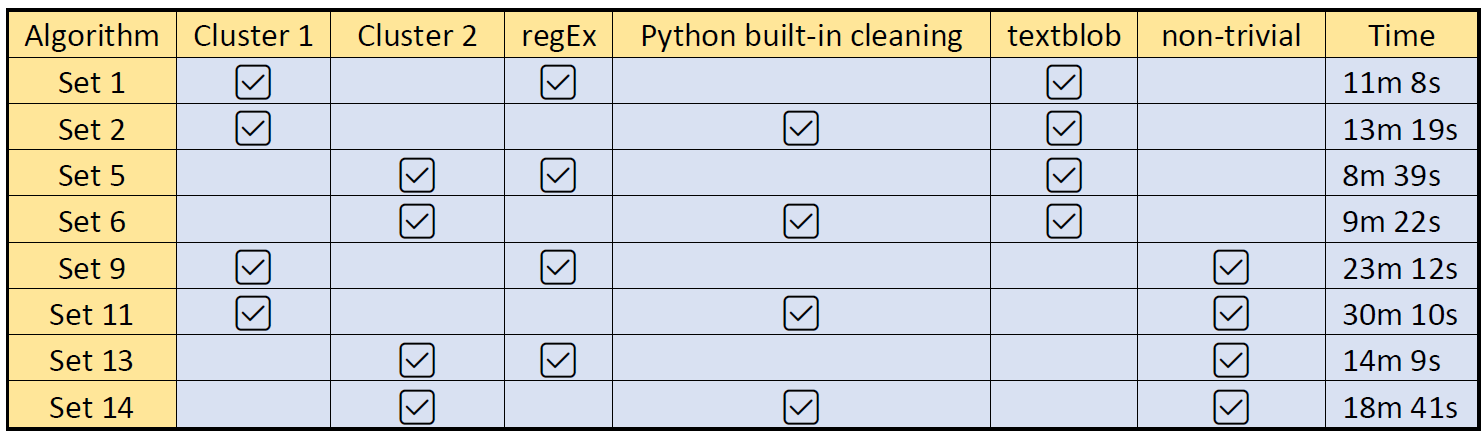
\includegraphics[width=\linewidth]{fig/sPerformance.png}
    \caption{Spark Performance statistics}
    \label{fig:sPerformance}
\end{figure}


\begin{figure}[t]
   \centering
   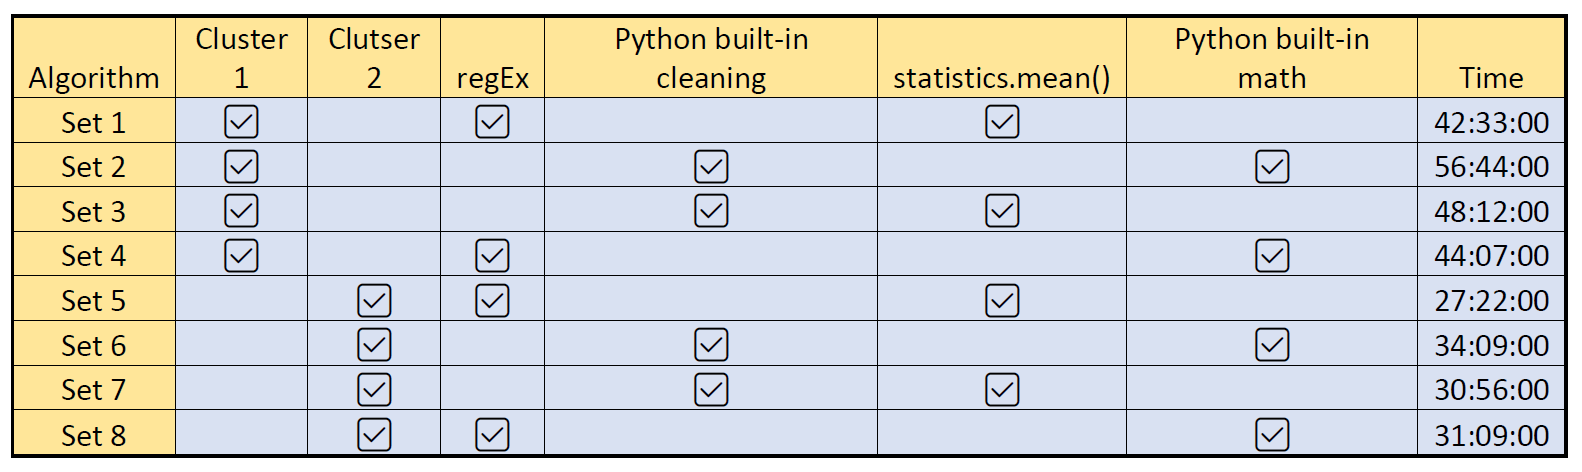
\includegraphics[width=\linewidth]{fig/hPerformance.png}
    \caption{Hadoop Performance statistics}
    \label{fig:hPerformance}
\end{figure}


\begin{figure}[t]
   \centering
   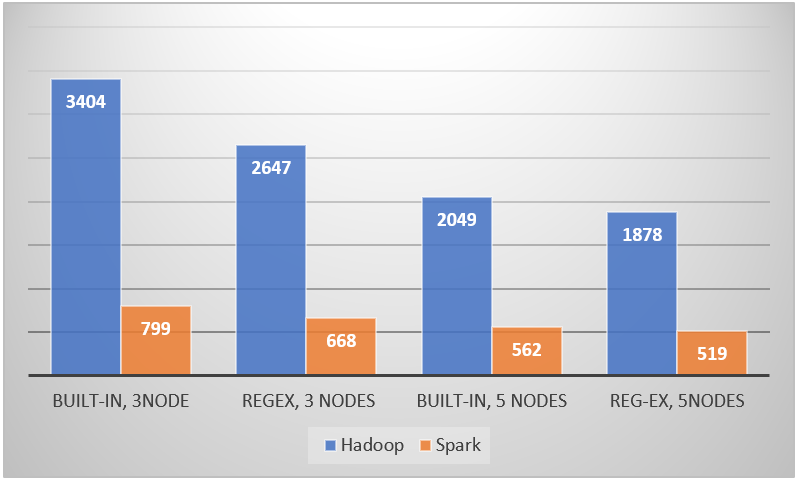
\includegraphics[width=\linewidth]{fig/hvss.png}
    \caption{Hadoop vs Spark}
    \label{fig:hvss}
\end{figure}


\bibliographystyle{ACM-Reference-Format}
\bibliography{citations.bib}

\end{document}
